\section{Уравнение равновесия в тяжелой среде}
\begin{align*}
  &\frac{1}{\rho(p)} \nabla p = \vec{f} \\
  &\nabla [\frac{1}{\rho(p)} \nabla p] = \nabla \cdot \vec{f}= -\nabla^2 \Pi \\
  &\vec{f} = -\nabla \Pi
\end{align*}

\begin{align*}
  &\nabla^2 \phi = - \epsilon_0 q\\
  &\vec{f}_{1, 2} = \frac{1}{4 \pi \epsilon_0} \frac{q_1 q_2 \vec{r}}{r^2 r} \\
  &\vec{f}_{1, 2} = -\gamma \frac{m_1 m_2}{r^2} \frac{\vec{r}}{r} \\
  &\nabla^2 \Pi = 4 \pi \gamma \rho \\
  &\nabla \cdot [ \frac{1}{\rho(p)} \nabla p] = -4 \pi \gamma \rho(p)
\end{align*}

Несжимаемая среда:
\[
  \rho = \rho_0 = const(p)
\]

\begin{defn}
  $\nabla^2 p = - 4 \pi \gamma \rho_0^2$ --- Уравнение Пуассона
\end{defn}

\begin{thm}[Обобщенная теорема Гаусса]
  \begin{figure}[h]
    \centering
    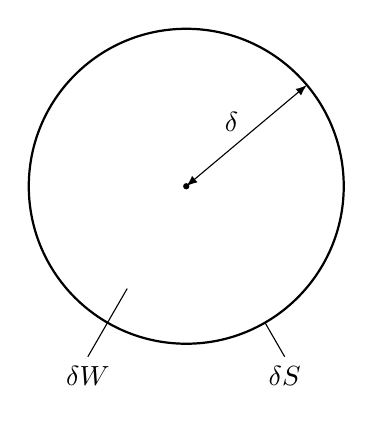
\begin{tikzpicture}
    \draw[thick] (0, 0) circle [radius=2];
    \fill (0, 0) circle [radius=.04];
    %\draw[<->] (2, 2) -- ++($ ({sqrt(3)/2}, 0.5) $);
    \draw[latex-latex] (0, 0) -- (40:2);
    \node at (55:1) {$\delta$};
    \draw (240:1.5) -- (240:2.5);
    \node[below] at (240:2.5) {$\delta W$};
    \draw (300:2) -- (300:2.5);
    \node[below] at (300:2.5) {$\delta S$};
\end{tikzpicture}

 
    \caption{Рассматриваемый шар обладает радиусом $\delta$, объёмом $\delta W$ и поверхностью $\delta S$}
  \end{figure}
  \begin{align*}
    &\int_W \nabla \otimes \ten{T} dW = \oint_S \vec{n} \otimes \ten{T} dS \\
    &\nabla \otimes T = \lim_{\delta W \to 0} \frac{1}{\delta W} \int_{\delta W} (\nabla \otimes \ten{T}) dW = \lim_{\delta W \to 0} \frac{1}{\delta W} \oint_{\delta S} \vec{n} \otimes \ten{T} d S\\
    & \nabla \cdot \vec{f} = \lim_{\delta W \to 0} \frac{1}{\delta W} \oint_{\delta S} \vec{n} \cdot \vec{f} d S\\
    &\nabla \cdot \vec{f} = \lim_{\delta \to 0} \frac{1}{\frac 43 \pi \delta^3} \oint_S -\gamma \frac{\rho \frac 43 \pi \delta^3}{\delta^2} \delta^2 dW = -\gamma \rho 4 \pi = -4 \pi \gamma \rho \\
    &\vec{f} = -\nabla \Pi \\
    &-\nabla^2 \Pi = - 4\Pi \gamma \rho\\
    &\nabla^2 \Pi = 4 \pi \gamma \rho\\
    &\nabla^2 \phi = -\epsilon_0 q
  \end{align*}
\end{thm}

\begin{figure}[h]
  \centering
  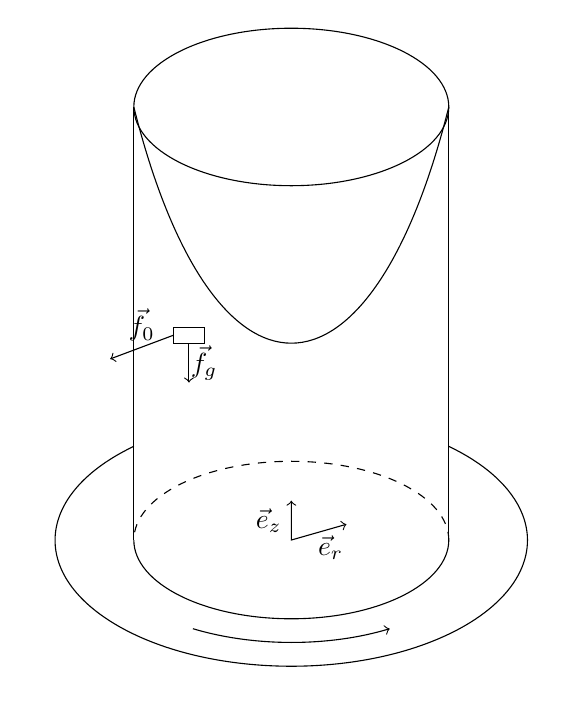
\begin{tikzpicture}
    \draw (-2, 2) coordinate (A) .. controls (-1, -2) and (1, -2) .. (2, 2) coordinate (B);
    \draw (A) -- (-2, -3.5);
    \draw (B) -- (2, -3.5);
    \draw (0, 2) ellipse (2 and 1);
    \draw[dashed] (2, -3.5) arc (0:180:2 and 1);
    \draw         (-2, -3.5) arc (180:360:2 and 1);
    \draw         (-2, -2.31) arc (131.8:408.2:3 and 1.6);
    \draw[<->] (0, -3) -- (0, -3.5) -- (.7, -3.3);
    \node[left] at (0, -3.25) {$\vec e_z$};
    \node at (0.5, -3.6) {$\vec e_r$};
    \draw[->] (0, -3.5)+(240:2.5 and 1.3) arc (240:300:2.5 and 1.3);

    \draw (-1.5, -1) rectangle +(.4,.2);
    \draw[->] (-1.3, -1) -- +(0,-0.5);
    \node[right] at (-1.4, -1.25) {$\vec f_g$};
    \draw[->] (-1.5, -0.9) -- +(-0.8, -0.3);
    \node[above] at (-1.9, -1.1) {$\vec f_0$};
\end{tikzpicture}

 
  \caption{На малый объём действует сила тяжести $\vec f_g$ и центробежная сила $\vec f_0$}
\end{figure}
\[
  \vec{F}_c = -m\omega^2 \vec{r}
\]


\begin{align*}
  &\vec{f}_g = \vec{g} = -g \vec{e}_z \\
  &\vec{f}_0 = \omega^2 \vec{r} = \omega^2 r \vec{e}_r \\
  &\vec{f} = \vec{f}_g + \vec{f}_0 = -g\vec{e}_z + \omega^2 r \vec{e}_r \iff \vec{f} = -\nabla \Pi \\
  &\Pi = gz - \frac{\omega^2r^2}{2} + C\\
  &\P = \int_{p_0}^p \frac{dp}{\rho(p)} = \int_{p_0}^p  \frac{dp}{\rho_0} = \frac{p - p_0}{\rho_0}\\
  &gz - \frac{\omega^2r^2}{2} + C + \frac{p - p_0}{\rho_0} = const \\
  &gz - \frac{\omega^2r^2}{2} + \frac{p}{\rho_0} = const
\end{align*}

Поверхность $p = p_A$
\begin{align*}
  &gz - \frac{\omega^2r^2}{2} + \frac{p_A}{\rho_0} = const \\
  &gz - \frac{\omega^2r^2}{2} = const \\
  &z(r) = \frac{\omega^2r^2}{2g} + C\\
  &V = \pi R^2 H \\
  &\int_0^R 2 \pi r z(r) dr
\end{align*}
